\section{Ainul Filiani (1174073)}
\subsection{Buku}
Belum Lunas 
\subsection{Pengertian Sistem Informasi Geografis}
\begin{enumerate}
\item definisi sistem informasi geografis 
Sistem Informasi Geografis atau disingkat SIG (bahasa Inggris Sistem Informasi Geografis (SIG) adalah sebuah komputer yang berbasis sistem informasi yang digunakan untuk menyediakan informasi bentuk digital dan menganalisis terhadap permukaan geografi bumi. Sistem Informasi Geografis (SIG) diartikan sebagai sistem untuk menyimpan, memantau, mengintegrasi, memanipulasi, menganalisis dan memaparkan data yang berkaitan dengan semua ruang yang terkait dengan keadaan bumi. Artikel yang berasal dari Prahasta yang membahas tentang GIS adalah menyimpan, membaca, mengintegrasi, memanipulasi, menganalisis dan memaparkan data yang berkaitan dengan semua ruang yang berkaitan dengan keadaan bumi., Informasi dan Sistem 
[1] dan dalam artikel dari Husein dkk, yang menyebutkan bahwa Sistem Informasi Geografis merupakan pemahaman dari Geografi Informasi dan Sistem [2].
karena Sistem Informasi Geografis adalah bidang kajian ilmu dan teknologi yang masih baru. Beberapa resolusi dari Sistem Informasi Geografis yaitu:
Definisi SIG menurut (Rhind, 1988) yaitu GIS adalah sistem komputer untuk mengumpulkan, memeriksa, mengintegrasikan dan menganalisis informasi yang berkaitan dengan permukaan bumi. 
Definisi SIG menurut (Marble dan Peuquet, 1983) dan (Parker, 1988: Ozemoy et al., 1981; Burrough, 1986) yaitu GIS berkaitan dengan data ruang-waktu dan sering tetapi tidak selalu, mempekerjakan perangkat keras dan perangkat lunak komputer.
SIG adalah suatu sistem yang dapat mengupayakan perangkat keras (perangkat keras), perangkat perangkat lunak (perangkat lunak), dan data, serta dapat digunakan dan digunakan sistem penyimpanan, pengolahan, serta analisis data yang dilakukan secara simultan, sehingga dapat diperoleh seluruh informasi yang dimuat langsung dengan aspek ke dalam ruangan.  SIG adalah manajemen data spasial dan data non-spasial yang berbasis komputer dengan menggunakan tiga karakteristik dasar, yaitu: 
\end{enumerate}
\begin{enumerate}
\item Memiliki fenomena yang aktual (data variabel non-lokasi) dan terkait dengan topik topik di lokasi penelitian 
\item merupakan suatu lokasi Tertentu 
\item Memiliki dimensi waktu.  Alasan GIS diperlukan karena data spasial ditanganinya sangat sulit karena peta dan data cepatnya kadaluarsa sehingga tidak ada layanan penyediaan data dan informasi yang diberikan menjadi tidak akurat
\end{enumerate}
Berikut merupakan keistimewaan analisa dengan sistem informasi geografis:
\begin{enumerate}
\item analisa proximity
\item analisa overlay
\end{enumerate}
\subsection{Sejarah}
Peta merupakan penggambaran grafis atau bentuk skala (mempertimbangkan) pada konsep tentang bumi dalam hal ini peta merupakan alat untuk melengkapi atau memuat tentang ilmu kebumian.  Bagaimana peta dahulu ditemukan?  Pengetahuan tentang dasar pembentukan sama seperti filsafat, yang mana sering dianggap berbeda.  Peta Menurut Claudius Ptolemaeus Ptolemy, Claudius Ptolemaeus yang dikenal dengan nama Ptolemy, hidup antara tahun 100 M dan 168 M, beliau merupakan salah satu sarjana sains pada masanya.  Dia tinggal dan bekerja di Alexandria, kota Mesir yang merupakan pusat Intelektual dunia barat dengan perpustakaan paling luas yang pernah diciptakan.  Ptolemy membawa semua pengetahuan dan keterampilan matematika dan astronomi dan menerapkannya pada pembuatan peta.  Dia memiliki daya tarik matematikawan dengan presisi untuk menunjukkan hubungan satu tempat ke tempat lain.  Berdasarkan perhitungan lingkaran dunia 18.000 mil, ia juga mengembangkan sistem grid latude dan bujur yang dirancang olehMarinus dari Tirus sementara beberapa rincian peta mungkin sedikit aneh dengan garis lintang sejajar dengan garis khatulistiwa dengan garis bujur yang membentang ke utara-selatan dengan busur anggun, sudah tidak tersedia  lagi bagi siapa saja yang pernah memiliki atlas.  Dalam persetujuan ini, Ptolemeus dapat membangun koordinat dan meminta lebih dari 8000 tempat koordinat masing-masing Bagi Ptolemeus, ini latihan matematik dan kita tidak akan pernah tahu apakah dia benar-benar membuat peta dari sini.
\subsection{koordinat}
Koordinat digunakan untuk menentukan titik di Bumi melalui garis lintang dan garis bujur.  Koordinat dibagi menjadi dua bagian irisan yaitu irisan melintang yang disebut dengan garis lintang mulai dari khatulistiwa, membesar ke arah kutub (utara maupun selatan) sedangkan yang lain membujur mulai dari garis Greenwhich membesar ke arah barat dan timur.  Koordinat ini ditulis dalam satuan derajat, menit, dan detik dan seterusnya. Untuk membagi dunia di dalam wilayah utara dan selatan, maka ditentukan garis yang tepat berada di tengah, yaitu garis Khatulistiwa atau Khatulistiwa. Untuk batas wilayah timur dan  barat, maka ditentukan sebuah garis Perdana meridian yang terletak di kota Greenwich (Inggris), dan perpotongannya bertemu di wilayah laut pasifik, yaitu memotong kepulauan Fiji.
\begin{itemize}

\item Garis Lintang 
Sebuah garis khayal yang digunakan untuk menentukan lokasi di Bumi terhadap garis khatulistiwa (utara atau selatan).  Posisi lintang merupakan penghitungan sudut dari 0 derajat di khatulistiwa sampai ke +90 derajat di kutub utara dan -90 derajat di kutub selatan.  Dalam bahasa Indonesia lintang di sebelah utara khatulistiwa diberi nama Lintang Utara (LU), demikian pula lintang di sebelah selatan khatulistiwa diberi nama Lintang Selatan (LS).  Lintang Utara dan Lintang Selatan menentukan sudut pandang antara posisi lintang dengan garis Khatulistiwa.  Garis Khatulistiwa sendiri adalah lintang 0 derajat.  Nilai koordinat lintang dimulai dari garis lingkaran khatulistiwa yang diberi nilai 0 derajat.  Selanjutnya garis lintang yang lain berbentuk lingkaran paralel (sejajar) khatulistiwa berada di sebelah utara dan selatan khatulistiwa.  Lingkaran paralel di selatan disebut garis lintang selatan (LS) dan diberi nilai negatif, sedangkan lingkaran paralel di utara diberi nilai positif dan disebut garis lintang utara.
\item Garis Bujur
Menggambarkan lokasi tempat di timur atau barat Bumi dari garis utara-selatan yang disebut Meridian Utama.  Bujur diberikan pada sudut pandang yang terdiri dari 0 derajat Meridian Utama ke +180 derajat Arah timur dan-180 derajat Arah barat Tidak seperti lintang yang memiliki ekuator sebagai posisi awal yang tidak memiliki posisi awal yang alami untuk perbatasan.  Bujur di sebelah barat Meridian diberi nama Bujur Barat (BB), demikian pula bujur di sebelah timur Meridian diberi nama Bujur Timur (BT).  Nilai koordinat garis bujur dimulai dari bujur 0 derajat yaitu Greenwhich, kemudian diperbesar ke arah timur dan barat sampai bertemu kembali di garis batas tanggal internasional yaitu terletak di selat bering dengan nilai 180 derajat.  Garis bujur 0 derajat disebut prime meridian atau meridian Greenwhich.  Garis bujur ke arah barat diberi nilai negatif dan disebut bujur barat (bujur barat) serta disingkat BB.  Sedangkan garis bujur yang ke arah timur diberi nilai positif dan disebut bujur timur (bujur timur) disingkat BT.  nilai koordinat atas yang disusun dari bujur 0 ke atas sesuai dengan pusat bumi.
\end{itemize}
\subsection{Data geospasial}
data raster adalah data yang tersimpan dalam bentuk grid atau petak jadi terbentuk pada sebuah ruang yang teratur dalam bentuk pixel (elemen gambar).  Foto digital seperti areal fotografi atau satelit merupakan bagian dari data raster pada peta.  Data raster memiliki kisi-kisi data terus. Diharapkan menggunakan gambar berwarna seperti fotografi, yang disetujui dengan tingkat merah, hijau, dan biru pada sel.  Data Raster (atau disebut juga dengan sel grid) merupakan data yang dihasilkan dari sistem penginderaan jauh.  Pada data raster.  Obyek geografis direpresentasikan sebagai struktur sel grid yang disebut dengan pixel (elemen gambar).  Pada data raster.  Resolusi (resolusi visual) tergantung pada ukuran pixelnya.  Dengan kata lain.  Resolusi piksel. Resolusi setiap kali bumi diwakili oleh setiap piksel pada citra.  Pada data raster, objek arsitektur direpresentasikan sebagai struktur sel grid yang disebut se-bagi pixel (elemen gambar).  Resolusi (resolusi visual) tergantung pada ukuran pixel-nya, semakin kecil ukuran permukaan bumi yang direpresentasikan oleh sel, semakin tinggi resolusinya.  Data Raster dihasilkan dari sistem penginderaan jauh dan sangat baik untuk merepresentasikan batas-batas yang berubah secara bertahap seperti jenis tanah, kelembaban tanah, suhu, dan lain-lain.
\subsection{link}
https://youtu.be/VtkOzHAdmk0
\subsection{plagiarisme}
\begin{figure}[H]
 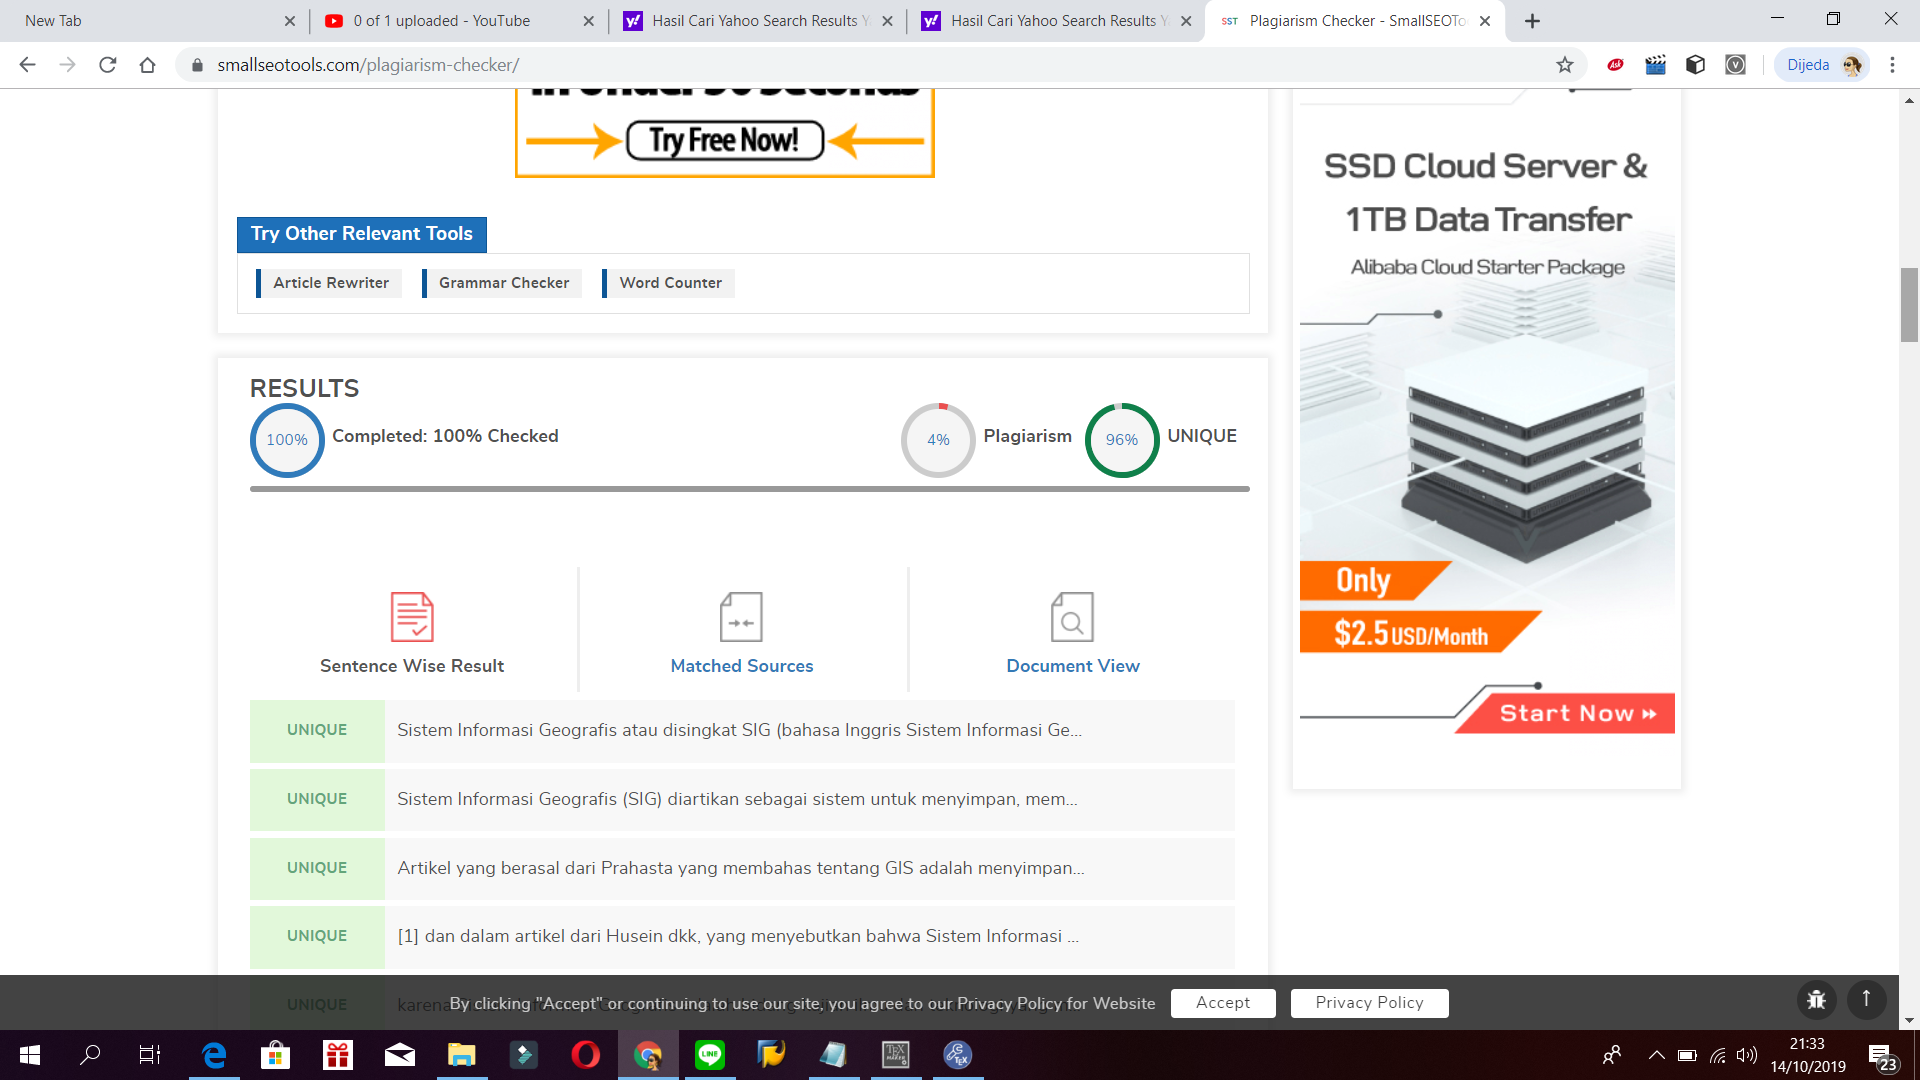
\includegraphics[width=4cm]{figures/Tugas1/1174073/plagiarism.png}
 \centering
 \caption{Gambar Plagiat}
\end{figure}